\documentclass[12pt]{article}

% Language setting
\usepackage[utf8]{inputenc}
\usepackage[bulgarian]{babel}

% --------------------- Packages  --------------------
% Use biblatex
\usepackage{biblatex}
\addbibresource{bibliography.bib}
% Table thickness
\usepackage{ctable}
% Equations: SI units
\usepackage{siunitx}
% Approximately equal
\usepackage{amssymb}
% degrees symbol
\usepackage{gensymb}
% warning box
\usepackage{pifont,mdframed}
% Multiline math
\usepackage{amsmath}

\newenvironment{warning}
  {\par\begin{mdframed}[linewidth=2pt, linecolor=white]%
    \begin{list}{}{\leftmargin=1cm
                   \labelwidth=\leftmargin}\item[\Large\ding{43}]}
  {\end{list}\end{mdframed}\par}

% --------------------- Title  --------------------
\addbibresource{bibliography.bib}

\begin{document}

% Anfang der Titelseite________________________________________________________________________________
\begin{titlepage}
	\flushleft
	{\scshape\Large Протокол X \hspace{2cm} Молекулна физика\par}
	\vspace{4cm}
	{\huge\bfseries Топлинно разширение на течности и твърди тела. Максимална плътност на водата\par}
	\vspace{1cm}
	{\LARGE\bfseries Лабораторно упражнение №3.8\par}
	\vspace{5cm}
    {\LARGE\bfseries Виолета Кабаджова, \par}
    {\large\bfseries ККТФ, фак. номер: 3PH0600026\par}
	\vspace{1cm}
	
	{\large Физически Факултет, 
	
	Софийски Университет "Св. Климент Охридски"
	
	18 май 2023 г.\par}
	
\end{titlepage}

\section{Теоритична част}\label{sec:theoretical-part}
Размерите на реалните физични тела променят размерите си, и съответно обема си с промяна на температурата. При твърдите тела това изменение може да бъде изотропно (във всички направления) или анизотропно (само в отделни напревления), докато при течности и газове то е единствено изотропно.
Големината на изменение на обема зависи от началната температура $T_0$ и от налягането $p$ и при фиксирано налягане се определя чрез производната $\left(\frac{\partial V}{\partial T}\right)_p$.

Относителносто изменение на обема се определя по формула \ref{eq:coefficient-of-thermal-expansion} и се нарича топлинен коефициент на обемно разширение $\beta$, $[\beta ]=K^{-1}$. При фиксирано налягане той числено е равен на разширението на единица обем при нарастване на температурата с един градус, като стойността му е най-малка за твърди тела и най-голяма за газове. Тъй като за течности и газове изменението на обема е назначително за промяна на температурата или налягането в малки граници, то записваме уравнение \ref{eq:coefficient-of-thermal-expansion} във вида \ref{eq:2-coefficient-of-thermal-expansion}.

\begin{equation}\label{eq:coefficient-of-thermal-expansion}
    \beta = \frac{1}{V}\left(\frac{\partial V}{\partial T}\right)_p
\end{equation}
 
\begin{equation}\label{eq:2-coefficient-of-thermal-expansion}
    \beta = \frac{1}{V}\frac{\Delta V}{\Delta T}
\end{equation}

\section{Експериментална част}

\subsection{Експериментална установка}
\begin{figure}
    \centering
    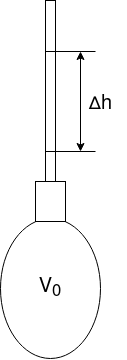
\includegraphics[width=0.15\textwidth]{images/set-up-thermal-expansion.drawio.png}
    \caption{\label{fig:setup}Схема на опитна постановка}
    \label{fig:setup}
\end{figure}

Експериментът изследва разширението на вода, налята в съд, подобен на представения в схема \ref{fig:setup}, към който има закрепена разграфена капилярка. Стъкленицата се пълни с вода до най-долното стъпало на скалата на капилярката, след което се загрява на водна баня, обемът на водата се разширява, при което се покачва нивото ѝ в капилярката, като разликата ѝ $\Delta h$ се отчита от скалата.

\subsection{Извеждане на работна формула}
Тъй като сечението на капилярката е с кръгла форма, обемът на височина $h$ се намира по формула \ref{eq:delta-h}.

\begin{equation}\label{eq:delta-h}
    \Delta V = S\Delta h = \pi r^2\Delta h    
\end{equation}

Освен течността в стъкленицата, самата стъкленица също се разширява при голяма температурна амплитуда с коефициент на обемно разширение $\beta_C$. Извеждаме работната ни формулата \ref{eq:beta} посредством формула \ref{eq:2-coefficient-of-thermal-expansion}, откъдето следва, че $\Delta V_T = \beta_T V_T \Delta T$, $\Delta V_C = \beta_C V_C \Delta T$.

\begin{equation}\label{eq:beta}
    \beta_T = \frac{1}{V\Delta T}(\beta_C V \Delta T + \pi r^2\Delta h)
\end{equation}

\subsection{Задача 1: Определяне обема на изследваната течност}
Масата на течността определяме по формула \ref{eq:mass}, където $m_1$ - масата на напълнената с вода стъкленица, $m_2$ - масата на празната стъкленица, $\rho$ - плътността на водата. Взимаме $\rho = 997 \frac{kg}{m^3}$. За $\Delta V$ взимаме в предвид единствено инструменталната грешка при измерване на масите: $\Delta V = (\frac{\Delta m_1}{m_1} + \frac{\Delta m_2}{m_2})$.

\begin{equation}\label{eq:mass}
    V = \frac{m_1 - m_2}{\rho} = (49.4 \pm 0.3 )\cdot 10^{-6} m^3
\end{equation}
\subsection{Задача 2: Измерване на коефициента на обемно разширение на дестилирана вода}
Поставяме измерителната клетка във водна баня, за да се загрее течността. След това цялата система се отстранява от нагревателя и се оставя да се охлажда (т.е. нивото на течността в капилярката да започне се понижава). Измерват се температурите на течността за всеки два милиметра разлика на капилярната скала и измерванията записваме в таблица \ref{tbl:results} и пресмятаме $\beta_T$ за всяка двойка.

\begin{table}[h]
\begin{center}
\begin{tabular}{|l|l|l|l|} \hline
    N & h_i, [mm] & T_i, [\deg C] & \beta_{Ti} \cdot 10^{-3}, [K^{-1}] \\ \hline
    0 & 80 & 56.5 & 0.40 \pm 0.04 \\ \hline
    1 & 78 & 55.6 & 0.44 \pm 0.05 \\ \hline
    2 & 76 & 54.8 & 0.34 \pm 0.04 \\ \hline
    3 & 74 & 53.7 & 0.26 \pm 0.02 \\ \hline
    4 & 72 & 52.1 & 0.27 \pm 0.03 \\ \hline
    5 & 70 & 50.6 & 0.56 \pm 0.06\\ \hline
    6 & 68 & 50 & 0.34 \pm 0.04 \\ \hline
    7 & 66 & 48.9 & 0.40 \pm 0.04 \\ \hline
    8 & 64 & 48 & 0.49 \pm 0.05\\ \hline
    9 & 62 & 47.3 & 0.44 \pm 0.05\\ \hline
    10 & 60 & 46.5 & 0.40 \pm 0.05\\ \hline
\end{tabular}
\caption{\label{tbl:results}Измервания и резултати}
\end{center}
\end{table}

На фиг. \ref{fig:chart} е представена зависимостта $\Delta h (\Delta T)$, от която определяме стойността на $\beta_T$ по графичен път посредством наклона на правата. Изчисляваме $\beta_T = \frac{dh}{dT} = 0.002$ и заместваме стойността във формула \ref{eq:beta}, която преобразуваме във вида, показан в уравнение \ref{eq:3-beta}, като получаваме $\beta_T = (0.37 \pm 0.01) \cdot 10^{-3} K^{-1}$. И на графиката, и таблично наблюдаваме отклонение спрямо останалите стойности около измервания 3, 4, 5. Заключваме, че в него момент са допуснати допълнителни човешки грешки по време на измерванията и е добре измерването да бъде повторено.  

\begin{equation}\label{eq:3-beta}
    \beta_T = \beta_C + \pi r^2 \frac{\Delta h}{\Delta T}
\end{equation}

\begin{figure}
    \centering
    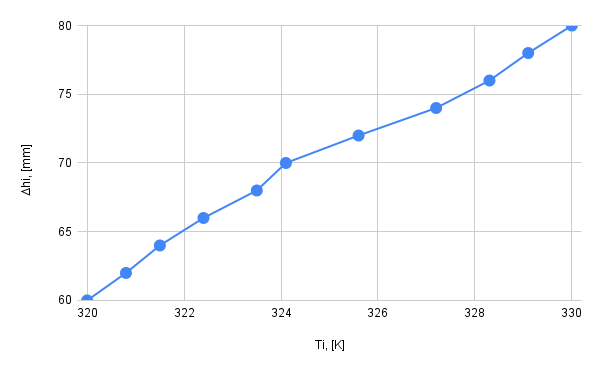
\includegraphics[width=0.8\textwidth]{images/chart.png}
    \caption{Зависимостта \Delta h (\Delta T)}
    \label{fig:chart}
\end{figure}

\end{document}
